%%%%%%%%%%%%%%%%%%%%%%%%%%%%%%%%%%%%%%%%%

% Journal Article
% LaTeX Template
% Version 1.3 (9/9/13)
%
% This template has been downloaded from:
% http://www.LaTeXTemplates.com
%
% Original author:
% Frits Wenneker (http://www.howtotex.com)
%
% License:
% CC BY-NC-SA 3.0 (http://creativecommons.org/licenses/by-nc-sa/3.0/)
%
%%%%%%%%%%%%%%%%%%%%%%%%%%%%%%%%%%%%%%%%%

%----------------------------------------------------------------------------------------
%	PACKAGES AND OTHER DOCUMENT CONFIGURATIONS
%----------------------------------------------------------------------------------------

\documentclass[twoside]{article}

\usepackage{lipsum} % Package to generate dummy text throughout this template


% deutsche Silbentrennung
\usepackage[ngerman]{babel}
% wegen deutschen Umlauten
\usepackage[utf8]{inputenc}
\usepackage[T1]{fontenc}

\usepackage[sc]{mathpazo} % Use the Palatino font
\usepackage[T1]{fontenc} % Use 8-bit encoding that has 256 glyphs
\linespread{1.05} % Line spacing - Palatino needs more space between lines
\usepackage{microtype} % Slightly tweak font spacing for aesthetics

\usepackage{amsmath}
\usepackage{mathtools}

\usepackage{eurosym}

%\usepackage[hmarginratio=1:1,top=32mm,columnsep=20pt]{geometry} % Document margins
% Margins
%\topmargin=-0.45in
%\evensidemargin=0in
%\oddsidemargin=0in
%\textwidth=7in
%\textheight=9.3in
%\headsep=0.25in
\usepackage[margin=0.7in]{geometry}

\usepackage{multicol} % Used for the two-column layout of the document
\usepackage[hang, small,labelfont=bf,up,textfont=it,up]{caption} % Custom captions under/above floats in tables or figures
\usepackage{booktabs} % Horizontal rules in tables
\usepackage{float} % Required for tables and figures in the multi-column environment - they need to be placed in specific locations with the [H] (e.g. \begin{table}[H])
   \def\deg{\ifmmode^\circ\else$^\circ$\fi}
   \usepackage{hyperref} % For hyperlinks in the PDF

   \usepackage{lettrine} % The lettrine is the first enlarged letter at the beginning of the text
   \usepackage{paralist} % Used for the compactitem environment which makes bullet points with less space between them

   \usepackage{abstract} % Allows abstract customization
   \renewcommand{\abstractnamefont}{\normalfont\bfseries} % Set the "Abstract" text to bold
   \renewcommand{\abstracttextfont}{\normalfont\small\itshape} % Set the abstract itself to small italic text

   \usepackage{titlesec} % Allows customization of titles
   \renewcommand\thesection{\Roman{section}} % Roman numerals for the sections
   \renewcommand\thesubsection{\arabic{subsection}} % Roman numerals for subsections
   \titleformat{\section}[block]{\large\scshape\centering}{\thesection.}{1em}{} % Change the look of the section titles
   \titleformat{\subsection}[block]{\large}{\thesubsection.}{1em}{} % Change the look of the section titles

%------ experiment
   \renewcommand\floatpagefraction{.9}
   \renewcommand\dblfloatpagefraction{.9} % for two column documents
   \renewcommand\topfraction{.9}
   \renewcommand\dbltopfraction{.9} % for two column documents
   \renewcommand\bottomfraction{.9}
   \renewcommand\textfraction{.1}   
   \setcounter{totalnumber}{50}
   \setcounter{topnumber}{50}
   \setcounter{bottomnumber}{50}
   \raggedbottom
%---- ende

   \titlespacing\section{0pt}{12pt plus 2pt minus 2pt}{4pt plus 2pt minus 2pt}
   \titlespacing\subsection{0pt}{8pt plus 2pt minus 2pt}{0pt plus 0pt minus 0pt}


   \usepackage{fancyhdr} % Headers and footers
   \pagestyle{fancy} % All pages have headers and footers
   \fancyhead{} % Blank out the default header
   \fancyfoot{} % Blank out the default footer
   \fancyhead[C]{Nautilus: Permafrostbeobachtung aus dem All $\bullet$ Februar 2014} % Custom header text
   \fancyfoot[RO,LE]{\thepage} % Custom footer text

   \setlength\parindent{0pt} % Removes all indentation from paragraphs


%----------------------------------------------------------------------------------------
%	TITLE SECTION
%----------------------------------------------------------------------------------------

   \title{\vspace{-15mm}\fontsize{24pt}{10pt}\selectfont\textbf{Kleinsatelliten Seminar: Team Nautilus}} % Article title

   \author{
%\large
      \textsc{Fries, Scherrmann, Huang, Leinbach, Cwielong} \thanks{Danke für die große Unterstützung durch die Betreuer am IRS}\\[2mm] % Your name
      \normalsize Universität Stuttgart - Institut für Raumfahrtsysteme \\ % Your institution
      \vspace{-5mm}
   }
   \date{}

%----------------------------------------------------------------------------------------

   \begin{document}

   \maketitle % Insert title

   \thispagestyle{fancy} % All pages have headers and footers

   \graphicspath{{images//}}

%----------------------------------------------------------------------------------------
%	ABSTRAKT
%----------------------------------------------------------------------------------------

   \begin{abstract}

      Im Rahmen des 'Kleinsatelliten Seminars' der Universität Stuttgart wurden in
      Teams zu je fünf Personen Phase 0/A (Design) Studien zur Umsetzung eines Kleinsatelliten mit
      der Hyperspektral Kamera (CHRIS) der Firma SSTL und einem Start mit der
      indischen PSLV durchgeführt. Dieser Bericht fasst die Ergebnisse des Teams
      ''Nautilus'' zusammen. Die Aufgabe umfasste die Definition einer primären
      Mission mit CHRIS sowie einer sekundären, selbst zu definierenden Mission. Aus den
      Missionen waren Top-Level, System und Subsystem Requirements abzuleiten, anhand derer
      der vollständige Satellitenbus auszulegen war.\\
      Nautilus primäre Mission ist die Erfassung des Rückgangs von Permafrost Böden.
      Seine Sekundäre Mission ist die Erprobung eines 3D-Gedruckten Hitzeschildes (ESA
      AMAZE) während des Wiedereintritts.


   \end{abstract}



%----------------------------------------------------------------------------------------
%	ARTICLE CONTENTS
%----------------------------------------------------------------------------------------

   \begin{multicols}{2} % Two-column layout throughout the main article text

%----------------------------------------------------------------------------------------
%	Einführung
%----------------------------------------------------------------------------------------

      \section{Einführung}

      \lettrine[nindent=0em,lines=3]{K} {\sc leinsatelliten}
      , also Satelliten unter 150 kg, 
      eignen sich ausgesprochen gut für Erdbeobachtung und universitäre Forschung. 
      Sie sind klein genug, um günstig auf einer großen Trägerrakete als Nebenlast 
      mitzufliegen, günstig genug, um von einem gut organisierten Institut entwickelt 
      und gebaut zu werden, und durch ihre geringen Trägheitsmomente und niedrige 
      Flughöhe exzellente Erdbeobachter. Um Studenten die Möglichkeit zu geben, ihr 
      Wissen zu erweitern und ihre Fähigkeiten und Qualifikation weiter zu 
      entwickeln, wird jährlich am Institut für Raumfahrtsysteme der Universität 
      Stuttgart das Kleinsatelliten Seminar durchgefüht. In diesem werden von kleinen, 
      studentischen Teams Phase 0/A(Design) Studien für Satelliten durchgeführt. 
      Im folgenden wird die Ausarbeitung des Projekts ''Nautilus'' zusammengefasst.
      \begin{figure}[H]
         \captionsetup{format=plain}
         \centering
         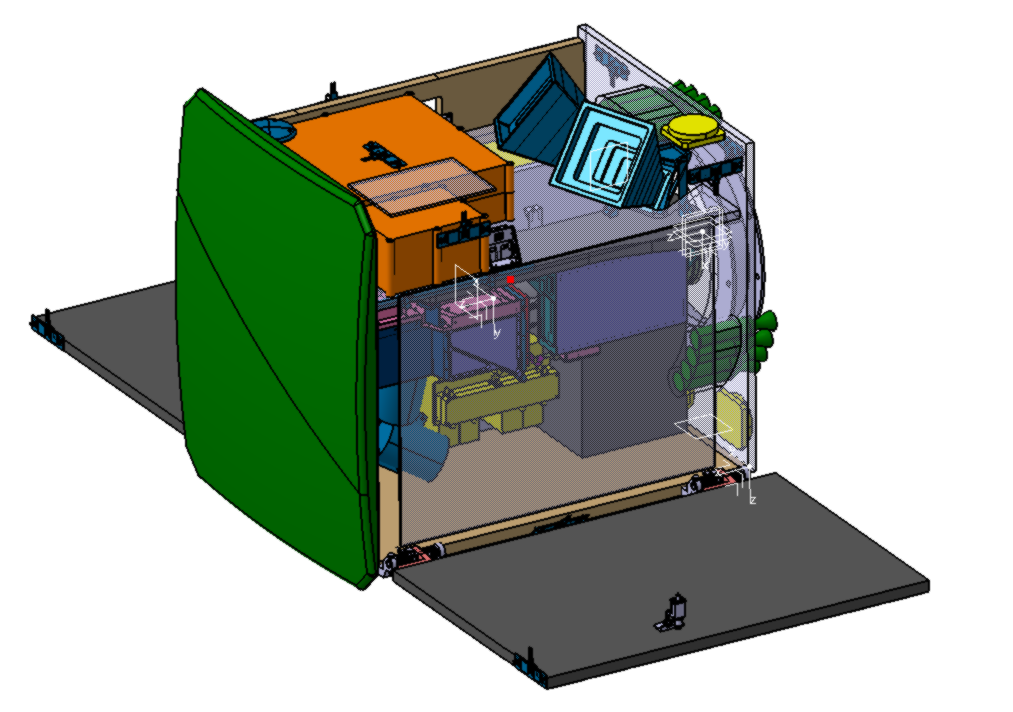
\includegraphics[width=\linewidth]{sat.png}       
         \caption{Kleinsatellit Nautilus}
      \end{figure}

%------------------------------------------------

%\subsubsection{CHRIS und das PSLV}

      \subsection{Primäre Mission: Permafrost}

      Das Abschmelzen von Permafrostböden\footnote{Permafrost: Boden, der länger als zwei
      Jahre durchgehend eine Temperaturen unter dem Gefrierpunkt von Wasser hatte.}
      durch die globale Erderwärmung ist ein zunehmendes Problem: In Permafrostböden
      sind große Mengen Methan und $CO_2$ gebunden, die durch das Abschmelzen freigesetzt werden. Diese Treibhausgase beschleunigen wiederum die globale Erderwärmung. Um quantitative Aussagen
      über den Abbau treffen zu können, wir Nautilus primäre Mission die
      Beobachtung und Qunatifizierung des Rückggangs von Permafrostböden betreffen.

      Permafrost lässt sich nur schwierig direkt beobachten, da elektromagnetische Strahlung nur bis zur halben Wellenlängen in den Boden eindringen kann.
      Er ist somit im Wellenlängenbereich von CHRIS nicht gut sichtbar. Die Vegetation auf 
      Permafrostböden hingegen lässt sich gut durch eine hyperspektrale
      Kamera beobachten. Diese variiert je nach Fortschritt des Tauvorgangs.

      Nautilus wird daher zuerst die Vegetation in polaren Regionen mit dem Push-Broom
      Verfahren abscannen. Nach anschließender Definition interessanter
      Regionen (am Boden) wird Nautilus diese beim nächsten Revisit im
      ''Target Pointing Mode''\footnote{Siehe hierzu auch: Geoscience and Remote Sensing Symbosium,
      2007, IGARSS 2007, IEEE international} erneut überfliegen und somit eine Klassifizierung der Vegetation erleichertn. Diese Messungen werden mit ''In-Situ''-Messungen
      kalibriert.

      \subsection{Sekundäre Mission: Wiedereintritt}

      Als sekundäre Mission soll das Großprojekt AMAZE\footnote{Additive Manufacturing
      Aiming towards Zero Emission} der ESA durch eine Technologie Erprobung
      unterstützt werden. AMAZE hat zum Ziel den 3D-Druck für Raumfahrtanwendungen
      interessanter zu machen. In diesem Rahmen wird versucht Materialien mit Schmelztemperaturen $ T_s
      \geq 3200\deg C $ durch Druckverfahren in gewünschte Bauteilformen zu bringen. Dies soll unteranderem das Drucken
      von Regulit auf dem Mond oder spezielle Metallegierungen auf der Erde
      ermöglichen. Nautilus wird ein gedrucktes Keramik Hitzeschild erproben. Dieses
      soll beim Wiedereintritt OnBoard durch Sensorik und OffBoard durch ein
      Beobachtungsflugzeug\footnote{als Referenz für die Machbarkeit gelten: Stardust,
      Hayabusa, ATV Jules Verne} optisch untersucht werden.

      \subsection{System Level Anforderunge}
      Tabellen \ref{tab:sysreq} und \ref{tab:misreq} stellen alle
      gegeben und daraus abgeleiteten System Requirements vor. Die Top-Level Requirements haben sich direkt aus der Aufgabenstellung ergeben.\\
%      \begin{table}[H]
%
%         \centering
%         \begin{tabular}{ll}
%%\cmidrule(r){1-2}
%            \toprule
%            R & Requirement \\
%            \midrule
%            1 & \parbox[t]{5cm}{Zwei-jährige Mission mit sstl CHRIS }  \\
%            %\midrule
%            2 & \parbox[t]{5cm}{Definition einer sekundären Mission  }  \\
%            %\midrule 
%            3 & Start mit dem PSLV  \\
%            %\midrule
%            4 & Kosten unter fünf M Euro  \\
%            %\midrule
%            5 & Ein Fehler Toleranz \\
%            \bottomrule
%         \end{tabular}
%         \caption{Requirements}
%         \label{tab:req}
%      \end{table}
      Allgemein gilt für alle Requirement Tabellen: Die erste Spalte 
      (falls vorhanden) referenziert die nächst höhere Requirement Ebene, auf die sich das aktuelle Requirement bezieht. Spalte zwei gibt dem Requirement auf seiner Ebene eine eindeutige Nummer. Spalte 3 enthält das Requirement in Prosa. Die Requirements sind nach folgendem Muster abgeleitet:\\
      Aufgaben Req. $\longrightarrow$ Mission Req. $\longrightarrow$ System Req. $\longrightarrow$ Subsystem Req.\\
      Aus der Tabelle \ref{tab:sysreq} werden in den Satellitenbus Sektionen dann die entsprechenden Subsystem Anforderungen abgeleitet.
      \begin{table}[H]
         \centering
         \begin{tabular}{ccl}
                 %\cmidrule(r){1-2}
            \toprule  
            MR & SR & System Requirement \\
            \midrule
            1 & 1 & \parbox[t]{5cm}{Der Orbit muss polare Regionen abdecken }  \\
                 %\midrule
            1 & 2 & \parbox[t]{5cm}{Der Satellitenbus muss mindestens zwei Jahre voll funktionieren }  \\
                 %\midrule
            1 & 3 & \parbox[t]{5cm}{Die wissenschaftlichen Ergebnisse müssen übertragen werden können}  \\
                 %\midrule
            2 & 4 & \parbox[t]{5cm}{Der Orbit Wiedereintritt nach <5 Jahren muss garantiert sein}  \\
                 %\midrule
            2 & 5 & \parbox[t]{5cm}{Gefährdung der Erdbewohner durch den Wiedereintritt muss ausgeschlossen werden }  \\
                 %\midrule
            2 & 6 & \parbox[t]{5cm}{Der Wiedereintritt soll einen wissenschaftlichen Mehrwert liefern }  \\
                 %\midrule
            3 & 7 & \parbox[t]{5cm}{Der Satellit darf nicht mehr als 150 KG wiegen}  \\
                 %\midrule
            3 & 8 & \parbox[t]{5cm}{Der Satellit darf PSLV Dimensionen nicht überschreiten}  \\
                 %\midrule
            3 & 9 & \parbox[t]{5cm}{Der Satellit muss die Lasten während des Launches überstehen}  \\
                 %\midrule
            4 & 10 & \parbox[t]{5cm}{Kosten dürfen fünf M Euro nicht übersteigen }\\
                 %\midrule
            5 & 11 & \parbox[t]{5cm}{Ein Fehler Tolerant}\\
            \bottomrule
         \end{tabular}
         \caption{System Requirements}
         \label{tab:sysreq}
      \end{table}

      \begin{table}[H]
         \centering
         \begin{tabular}{ccl}
            \toprule
            R & MR & Mission Requirement \\
            \midrule
            1 & 1 & \parbox[t]{5cm}{Beobachtung der Vegetation auf Permafrostböden }  \\
            %\midrule
            2 & 2 & \parbox[t]{5cm}{Erprobung eines 3-D gedruckten Hitzeschildes  }  \\
            %\midrule
            3 & 3 & Start mit dem PSLV  \\
            %\midrule
            4 & 4 & Kosten unter fünf M Euro \\
            %\midrule
            5 & 5 & Ein Fehler Toleranz \\
            \bottomrule
         \end{tabular}
         \caption{Mission Requirements}
         \label{tab:misreq}
      \end{table}
%----------------------------------------------------------------------------------------
%	Satellitenbus
%----------------------------------------------------------------------------------------

      \section{Satellitenbus}
      \subsection{Orbit}

      SSR 1 erfordert einen Orbit mit hoher Inklination. SSR 2 ist mit Bodenstationen in Japan und Deutschland für beinahe jeden Orbit gegeben.
      SSR 3 benötigt eine möglichst niedrige Start Altitude, SSR 4 benötigt eine Höhe über 400 km. Um dies für zwei Jahre zu garantieren, wurde ein sonnensynchroner Orbit mit den Eigenschaften beschrieben in Tabelle \ref{tab:orbit} ausgewählt.
      \begin{figure}[H]
         \captionsetup{format=plain}
         \centering
         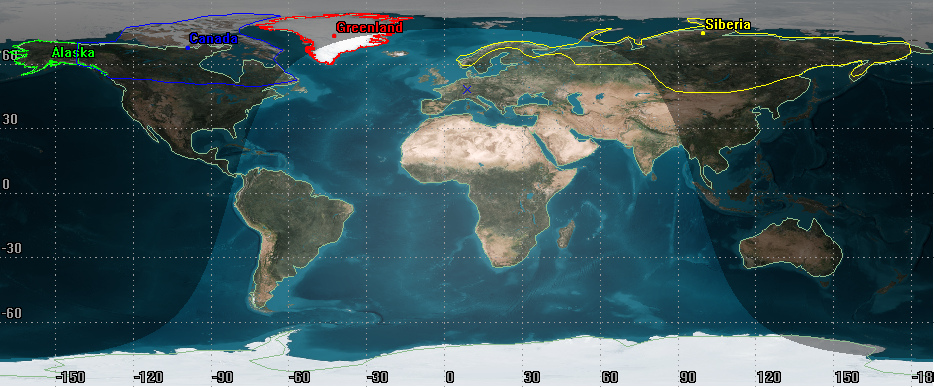
\includegraphics[width=\linewidth]{Coverage.png}       
         \caption{Beobachtungsgebiete zur Charakterisierung der Permafrost Entwicklung. (\textit{Source:} STK 10)}
      \end{figure}
      \begin{table}[H]
         \centering
         \begin{tabular}{ccl}
            \toprule
                  %\cmidrule(r){1-2}
            SR & SSR. & Sub System Requirement \\
            \midrule
            1 & 1 & \parbox[t]{5cm}{Polare Regionen müssen voll abgedeck sein}  \\
                  %\midrule
            3 & 2 & \parbox[t]{5cm}{Kontakt zu Bodenstationen muss ausreichend sein für Payload-Downlink}  \\
                  %\midrule
            4 & 3 & \parbox[t]{5cm}{Die Zeit bis zum Wiedereintritt muss weniger als 5 Jahre betragen}  \\
                  %\midrule
            2 & 4 & \parbox[t]{5cm}{Ausreichende Auflösung der Kamera in den ersten zwei Jahren}  \\
            \bottomrule
         \end{tabular}
         \caption{Orbit Requirements}
         \label{tab:orbreq}
      \end{table}

      Dieser resultiert in keiner direkten Überlappung der Schwade und ermöglich eine Abdeckung von 94\% der zu beobachtenden Fläche in etwa acht Wochen (STK-Analyse).
      \begin{table}[H]
         \centering
         \begin{tabular}{ll}
            \toprule  
            Parameter & Wert \\
            \midrule
            Höhe [km] & 450   \\
                  %\midrule
            Inklination $[\deg]$ & $97.2\deg$  \\
                  %\midrule 
            LTDN [hh:mm] & 10:15\\
                  %\midrule
            Orbitperiode [min] & 92.6\\
                  %\bottomrule 
            Revisit Zeit [d] & ~14 \\
                  %\midrule 
            Schwadbreite [km] & 20.44 \\
                  %\midrule 
            GSD$_y$ [m] & 27.23\\
            \bottomrule
         \end{tabular}
         \caption{Orbit Parameters}
         \label{tab:orbit}
      \end{table}

      \subsection{OBDH}

      Tabelle \ref{tab:obdhreq} zeigt alle SS Requirements. Um SSR 2 und
      SSR 4 zu genüge zu kommen, wird die Payload unabhängig vom OBC betrieben.
      Dazu wird das OBDH in einen OBC und eine Payload Unit mit Payload Computer
      und Mass Memory Unit aufgespalten. Der OBC betreibt den Satellitenbus, die PLU 
      die Payloads. Damit SSR 4 erfüllt ist, wird der OBC kaltredundant verbaut und
      kann durch die PCDU, die auch ans TTC angeschlossen ist, neugestartet werden.
      Als OBC wird der kommerzielle OBC 750 von SSTL verwendet (SSR2). Um mit dem
      Bus kommunizieren zu können, wird ein extra IO-FPGA-Board verbaut. Für CCSDS
      wird ein extra CCSDS Board verbaut. Beide Boards sind über SpaceWire verbunden
      und kaltredundant in einer Box verbaut (IO-Hub). 
      \begin{figure}[H]
         \captionsetup{format=plain}
         \centering
         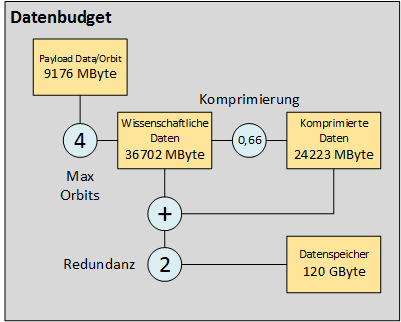
\includegraphics[width=\linewidth]{Datenbudget.png}       
         \caption{Berechnung des Datenbudgets. Hauskeeping Daten speichert der OBC direkt.}
         \label{fig:databudget}
      \end{figure}
      Die PLU besteht aus zwei mal jeweils einem Payload Computer FPGA mit je 4
      MM-Boards, die jeweils 15 GB NAND Flash enthalten (SSR 1).
      Somit ist es intern Kaltredundant (SSR 4). Die Payload und der Downlink
      Transmitter sind direkt an die PLU angeschlossen. Der PLC kann mit
      unterschiedlichen Betriebssystem für die jeweiligen Modi gestartet
      werden (Nadir-Pointing, Target Pointing, Downlink, Reentry, Komprimierung),
      um in jedem Modus minimal Strom zu verbrauchen. Der Payload FPGA verfügt
      über ein Programm zur 1,5 Fachen Komprimierung (SSR 3). 
      Figur ref{fig:databudget} zeigt das Datenbudget.

      \begin{table}[H]
         \centering
         \begin{tabular}{ccl}
            \toprule  
            SR & SSR. & Sub System Requirement \\
            \midrule
            3 & 1 & \parbox[t]{5cm}{Es muss genügend Speicherplatz für alle Daten vorhanden sein}  \\
            %\midrule
            6 & 2 & \parbox[t]{5cm}{Der OBC muss bis nach dem Wiedereintrtt funktionsfähig sein}  \\
            %\midrule
            3 & 3 & \parbox[t]{5cm}{Payload Daten müssen für den Downlink aufbereitet werden}  \\
            %\midrule
            11 & 4 & \parbox[t]{5cm}{Muss ein Fehler Tolerant sein}  \\
            %\midrule
            10 & 5 & \parbox[t]{5cm}{Kosten und Stromverbrauch sind minimal zu halten}  \\
            \bottomrule
         \end{tabular}
         \caption{OBDH Requirements}
         \label{tab:obdhreq}
      \end{table}


      \subsection{De-Orbit}      
      Tabelle \ref{tab:doreq} die Anforderungen an den Wiedereintritt.
      SSR 1 fordert einen Ausschluss der Gefährdung für Erdbewohner durch den Wiedereintritt.
      Dies kann auf auf zwei Weisen gewährleistet werden:
      \begin{enumerate}
         \item Die Sicherstellung des vollständigen Demise des Satelliten.
         \item Einen aktiven Wiedereintritt.
      \end{enumerate}
      Punkt 2. gibt zusätzlich die Möglichkeit der Beobachtung von einem Beobachtungsflugzeug.
      Ein Tradeoff zwischen aktivem und passivem Wiedereintritt sowie der Möglichen aktiven 
      Wiedereintritts Möglichkeiten ergibt eine eindeutige Vorteile des aktiven Wiedereintritts.
      Der aktive Wiedereintritt wird durch EPS(Electric Smart Propulsions) Feststoff Booster 
      der Firma DSSP(Digital Solid State Propuslions) umgesetzt. Dies sind elektrisch zünbare 
      Mini-Booster mit einem für Feststoffe typischen Isp.
      Da der Satellit Massenbeschränkt ist (SSR 3), sollte so wenig wie möglich Treibstoff Masse
      mitgenommen werden. Ein Kompromiss zwischen SSR1 und SSR3 führt auf ein De-Orbit Manöver
      in einer Höhe von ca 150km. Dies senkt die Treibstoffmasse genug, damit der Satellit
      realisierbar bleibt, lässt aber genug spiel, um das De-Orbit Manöver aktiv auf ein angestrebtes
      Ziel zu steuern.


      \begin{table}[H]
         \centering
         \begin{tabular}{ccl}
            \toprule  
            SL. & SSR. & Sub System Requirement \\
            \midrule
            5 & 1 & \parbox[t]{5cm}{Der Wiedereintritt darf keine Gefahr für Erdbewohner darstellen}  \\
            %\midrule
            9 & 2 & \parbox[t]{5cm}{Mögliche De-Orbit Triebwerke müssen PSLV verträglich sein}  \\
            7 & 3 & \parbox[t]{5cm}{Der Satellit muss weniger als 150 KG wiedegen}  \\
            \bottomrule
         \end{tabular}
         \caption{De-Orbit Requirements}
         \label{tab:doreq}
      \end{table}


      Die Booster sind in drei Viererpacks auf der Unterseite des Satelliten angebracht. 
      Dadurch kann ihr Schub durch den Schwerpunkt des Satelliten wirken und ungewollte Drehungen 
      verhindert werden. Durch das Ausbrennen des Treibstoffes wandert der Schwerpunkt des 
      Satelliten in Richtung Hitzeschild und damit in eine bessere Lage für einen stabilen 
      Wiedereintritt. Nach dem De-Orbit-Manöver muss der Satellit noch gedreht werden. Das 
      ACS System ist in dem verbleibenden Zeitfenster bis zu den spürbaren Auswirkungen  
      der Atmosphäre dazu imstande.
      Die Booster werden durch ein Steuergerät von der Firma DSSP gesteuert, das die benötigte 
      Leistung durch Kondensatoren sammelt und temporär bereitstellt.

      \subsection{TPS}
      Um SSR2 zu erfüllen, müssen zuerst die thermischen Lasten bekannt sein.
      Simulationen mit ASTOS liefern hierfür hinreichende Näherungen. Figur \ref{fig:astos}
      zeigt den Verlauf der Wärmefluss Dichte und der Flughöhe über der Zeit.
      Die Wärmefluss Dichte hat ihre Spitze bei ca. $600 W/m^2$. Hieraus lässt sich die 
      maximale Wandtemperatur ungefähr über eine Wärmefluss Billianz errechnen:
      \begin{align}
         \dot q_{Gesamt} &= 0 = \dot q_{reentry} - \dot q_{radian} \\
         \dot q_{radiation} &= \epsilon * \sigma * T_{wall}^4 \\
         T_{wall} &= (\frac{\dot q_{reentry}}{\epsilon*\sigma})^{1/4} 
      \end{align}
      Die Temperaturen, die unser Satellit aushalten muss, werden so bisher nur von
      ablativen Hitzeschilden und Keramiken ausgehalten. Ablative Hitzeschild können
      nicht gedruckt werden, daher wird für die Mission ein keramisches Hitzeschild
      verwendet. Als Grundlage für die Auslegung dienen die schwarzen Keramik-Kacheln
      des Space Shuttles. 
      \begin{table}[H]
         \centering
         \begin{tabular}{ccl}
            \toprule  
            SL. & SSR. & Sub System Requirement \\
            \midrule
            6 & 1 & \parbox[t]{5cm}{Am TPS sollen Messungen durchgeführt werden}  \\
            %\midrule
            6 & 2 & \parbox[t]{5cm}{Der Satellit soll den Wiedereintrtt überstehen}  \\
            \bottomrule
         \end{tabular}
         \caption{TPS Requirements}
         \label{tab:tpsreq}
      \end{table}
      Als TPS wird somit eine SiC Keramik mit einer Dicke von ca. 4 mm verwendet.
      Dahinter befindet sich eine ca 30mm dicke Schicht aus Aluminiumoxid 
      $Al_2O_3$ Schaum-Keramik. Diese ist über Standoffs mit der klaten Aluminium Struktur
      des Satelliten verbunden. Dies liefert einen hinreichenden Hitzeschutz.
      Das TPS muss im Staupunkt verstärkt werden: Hier wirken die größten Lasten.
      Alle Kanten müssen stark abgerundet sein. Auch die Kanten müssen verstärkt werden,
      da im Hyperschall an kleinen Radien sehr hohe thermische Lasten wirken.
      Zur Instrumentierung wird das Hitzeschild mit 15 paar Thermoelementen und 15
      Druckports versehen.    
      \begin{figure}[H]
         \captionsetup{format=plain}
         \centering
         \includegraphics[width=\linewidth]{ort.jpg}       
         \caption{Wiedereintrittsort: Siera Nevada.}
         \label{fig:enter}
      \end{figure}    
      \begin{figure}[H]
         \captionsetup{format=plain}
         \centering
         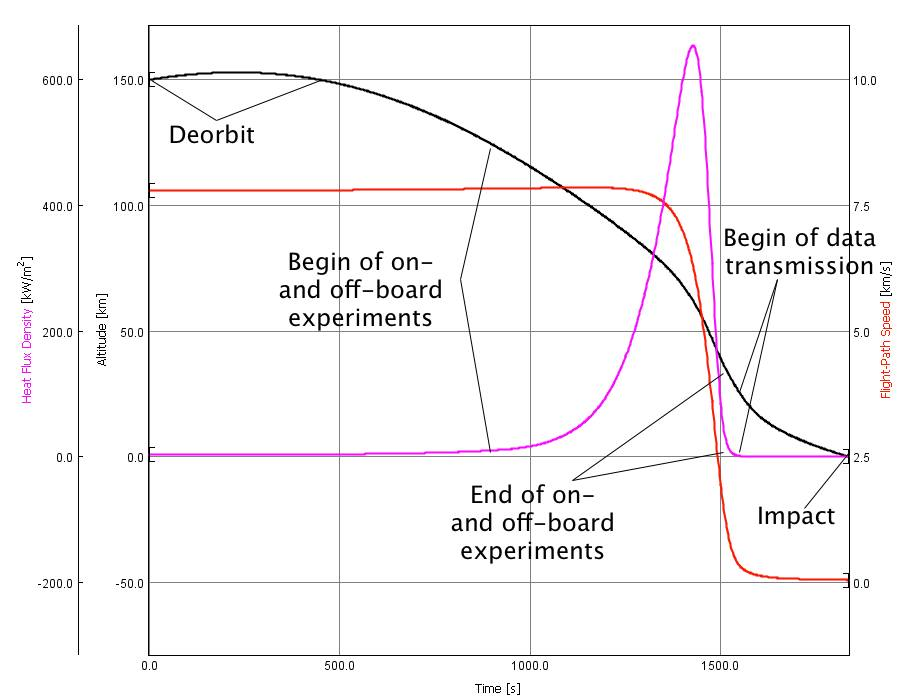
\includegraphics[width=0.8\linewidth]{astos.jpg}       
         \caption{Thermische Lasten und Zeitablauf des Wiedereintritts.}
         \label{fig:astos}
      \end{figure}    


      Die Thermoelemente werden jeweils paarweiße in unterschiedlicher
      Tiefe in der Isolation angebracht. Für die Druckports werden sehr kleine Löcher in das
      Hitzeschild gebohrt. Figur \ref{fig:positioning} zeigt die Positionen der Messsonden.
      Wie zu erkennen ist, sind diese in den Hauptachsen sowie der Diagonalen angebracht.
      Dies ermöglicht im Falle eines stabilen Wiedereintritts das erstellen eines
      genauen Temperatur und Druck Profils. Die Verteilung der Druckports ermöglicht
      gleichzeitig auch aussagen über die Stabilität des Wiedereintritts.
      Die verwendeten Messsonden sind Thermoelemente (Omega P30R (Type B)) und Drucksensoren
      (Measurement Specialties EPIH), wie sie auch für die 
      Mirka 2 Wiedereintritssprobe geplant sind. Über den interessanten Messzeitraum
      ergibt sich insgesamt eine Messdaten Menge von 365KB. Diese soll über ein 
      Relay durch die IRIDIUM Konstellation an das IRS übertragen werden.

      Zusätzlich zu den On-Board Messungen sollen Off-Board Messungen von einem
      Beobachtungsflugzeug aus stattfinden. Ein Beispiel für mögliche Instrumentierung
      wäre das am IRS entwickelte SLIT. Die genauen Instrumente an Board des Flugzeuges
      müssen in der weiteren Entwicklungs und Planungsphase noch genau definiert werden.

      \begin{figure}[H]
         \captionsetup{format=plain}
         \centering
         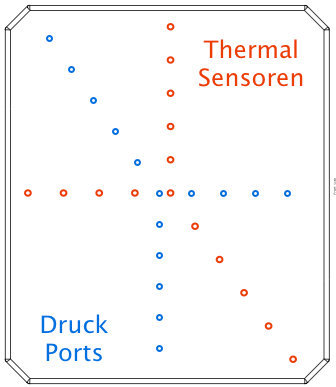
\includegraphics[width=0.5 \linewidth]{Einbau.png}       
         \caption{Positionen der Sensorik im Hitzeschild.}
         \label{fig:positioning}
      \end{figure}   




      \subsection{ACS}
      Beim ACS wurde darauf geachtet, die Requirements die beschrieben und berechnet worden 
      sind zu erfüllen. Um die Drei-Achsen-Stabilisierung zu erreichen wurden Reaktionsräder benötigt.

      Die Magnetorquer wurden benötigt um die Raktionsräder zu entdrallen.
      Diese wiederum haben Magnetometer benötigt um das Erdmagnetfeld zu messen.
      Die zu erreichende ''Pointing Knowledge'' wird durch Star Tracker realisiert.
      Die Drehrate die durch eine Simulation ermittelt wurden ist, 
      war zu hoch für die Auflösung der Star Tracker. Deshalb wurde noch eine IMU
      benötigt. Für den ''Safe Mode' sind die bisherigen Instrumente zu Energieintesiv.
      Da noch eine Ausrichtung zur Sonne im ''Safe Mode'' sichergestellt werden musste,
      wurde noch Sonnensensoren eingeführt.
      \begin{table}[H]
         \centering
         \begin{tabular}{ccl}
            \toprule  
            SL. & SSR. & Sub System Requirement \\
            \midrule
            2 & 1 & \parbox[t]{5cm}{Das ACS muss den Satellit nach dem Aussetzen stabilisieren können}  \\
            %\midrule
            3 & 2 & \parbox[t]{5cm}{Eine Pointing Knowledge von 11.92'' ist benötigt}  \\
            %\midrule
            2 & 3 & \parbox[t]{5cm}{Ein Pointing Accuracy von 238.549'' ist benötigt}  \\
            %\midrule
            4 & 4 & \parbox[t]{5cm}{Der Satellit muss drei-Achsen-stabilisiert sein}  \\
            %\midrule
            11 & 5 & \parbox[t]{5cm}{Das ACS muss ein Fehler Tolerant sein}  \\
            %\midrule
            9, 10 & 6 & \parbox[t]{5cm}{Der beste Kompromiss aus Leistung, Gewicht und Kosten und Stromverbrauch sollte verwendet werden}  \\
            \bottomrule
         \end{tabular}
         \caption{ACS Requirements}
         \label{tab:acsreq}
      \end{table}

      \subsection{TT\&C und Payload Downlink}
      Das TTC wird im kommerziellen S-Band über einen Transceiver von
      \textit{STT-Systemtechnik} realisiert mit Patch Antennen von \textit{SSTL}.
      Ein heißredunanter Empfänger stellt sicher das Verfügbarkeit immer gegeben ist.\\
      Der Downlink der enormen Datenmengen von CHRIS (137Mbps mit 1.5-facher,
      verlustfreier Kompression) erfolgt im X-Band \footnote{Vgl. Proba V
      Downlink} mit einer selbst entworfenen Hornantenne \footnote{Es
         wurde das Auslegungsprogramm \textit{Antenna Magus} verwendet}
         und einem Transmitter von \textit{SSTL}. Die Bodenstation am IRS müsste
         dafür noch aufgerüstet werden, es wird jedoch auch die Kooperation mit
         der Tohoku Universität in Japan genutzt, die bereits über X-Band Fähigkeiten
         verfügt. Darüber hinaus könnten Bodenstationen des \textit{ESTRACK}-Netzwerks,
         durch die Kooperation mit ESA, zeitweise zur Verfügung stehen.
         Die mittlere Kontaktzeit zur IRS-Bodenstation beträgt \textasciitilde 6min\\
         Durch die Benutzung von herkömmlichen \textit{Iridium} Transceivern und Patch 
         Antennen im L-Band is sichergestellt, dass alle Informationen während des
         Wiedereintritts übertragen werden können. Diese Komponenten müssen 
         allerdings noch auf Weltraumtauglichkeit getestet und ggf. modifiziert werden).\\
         Eine Margin von $3dB$ beim Signal-Rauschanbstand wird in keinem Fall unterschritten.
         \begin{table}[H]
            \centering
            \begin{tabular}{ccc}
               \toprule  
               Band & Freq. [MHz] & Datenrate [Mbps]\\
               \midrule
               S (Down) & 2200 - 2290 & 133.3 \\
               S (Up) & 2025 - 2110 & 62.96 \\
               X & 8050 - 8150 & 148.15 \\
               L & 1616 - 1626.5 & 7.78 \\
               \bottomrule
            \end{tabular}
            \caption{Gewählte Bänder und max. Übertragungsraten}
            \label{tab:ttcconfig}
         \end{table}
         Redundanzen in allen vorgestellten Kommunikationsystemen verhindern 
         das Auftreten eines Single-Point Fehlers.
%            \begin{table}[H]
%               \centering
%               \begin{tabular}{ccl}
%                  \toprule  
%                  SL. & SSR. & Sub System Requirement \\
%                  \midrule
%                  x & 1 & \parbox[t]{5cm}{Der Satellit muss immer erreichbar sein}  \\
%                  %\midrule
%                  3 & 2 & \parbox[t]{5cm}{Alle Payload Daten müssen übertragbar sein}  \\
%                  %\midrule
%                  6 & 3 & \parbox[t]{5cm}{Die Daten der sekundären Nutzlast müssen an die IRIDIUM Konstellation gesendet werden köennen}  \\
%                  %\midrule
%                  11 & 4 & \parbox[t]{5cm}{Muss 1 Fehler Tolerant sein}  \\
%                  \bottomrule
%               \end{tabular}
%               \caption{TT\&C Requirements}
%               \label{tab:ttcreq}
%            \end{table}


         \subsection{EPS}
         Das Energiesystem besteht aus drei Solarpaneelen bestück mit insgesamt 360 \textit{Azurspace TJ 3G30C-Advanced} Solarzellen, wobei die 30 parallel geschalteten Strings jeweils aus 12 in Reihe geschalteten Zellen bestehen. Die Batterie besteht aus 5 parallelen Strings mit jeweils 8 in Reihe geschalteten \textit{Saft VES-16}. Die Auslegung erfolgte über den schlecht möglichsten Betriebsfall, Abb. \ref{fig:fail}, und einer Margin von 20\%. Die nicht senkechte Ausrichtung zur Sonne, während Downlink und Aufnahmen, wurde berücksichtigt.\\
         Beim Start des Satelliten sind die Batterien zu max. 65\% geladen. Im schlimmsten Fall würde dies zu einer einmaligen Entladungstiefe von 35\% am Ende des Deployments führen (Gesamtdauer ca. 175min). Ablauf siehe Abb. \ref{fig:deploy}.\\
         Es wurde ein Shunt reguliertes DET System gewählt und die PCDU arbeitet unreguliert, was an jedem elektrischen Bauteil einen zusätzlichen DC/DC Konverter erforderlich macht. Die Vorteile sind niedrigere Masse, weniger Teile und eine insgesamt höhere Pfadeffizienz. Die max. Gesamtleistung der Solarpaneele am BOL beträgt $\sim 196 Watt$, die der  Batterien $648Wh$. Ein DoD von 20\% wird außer während Deployment und Wiedereintritt, nicht überschritten.     
         Selbst beim Ausfall eines kompletten Paneels ist sichergestellt, dass die durchschnittlich aufgenommene Energie ausreicht, um die Mission durchzuführen. Lediglich die Batterie wird mehr beansprucht, was aber kein Problem darstellt. 
         \begin{figure}[H]
            \captionsetup{format=plain}
            \centering
            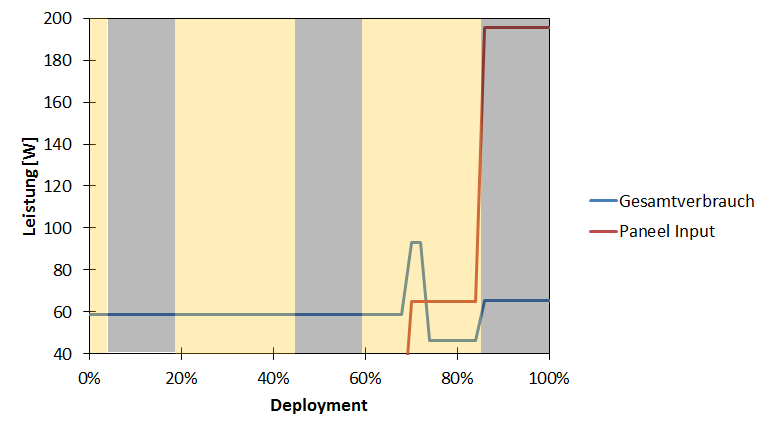
\includegraphics[width=\linewidth]{Deployment.png}       
            \caption{Ablauf des Deployments. Dunkle Stellen sind Schattenzeiten. Helle Sonnenzeiten.}
            \label{fig:deploy}
         \end{figure}
         Darüber hinaus sind die einzelnen Strings auf den Paneelen mit der \textit{Vectronics} PCDU so verschaltet, dass beim Ausfall eines Strings, nicht das ganze Paneel ausfällt. Die PCDU ist darüber hinaus mit dem TTC System verbunden und kann selbstständig den Onboard Computer neu starten.\\
         \begin{figure}[H]
            \captionsetup{format=plain}
            \centering
            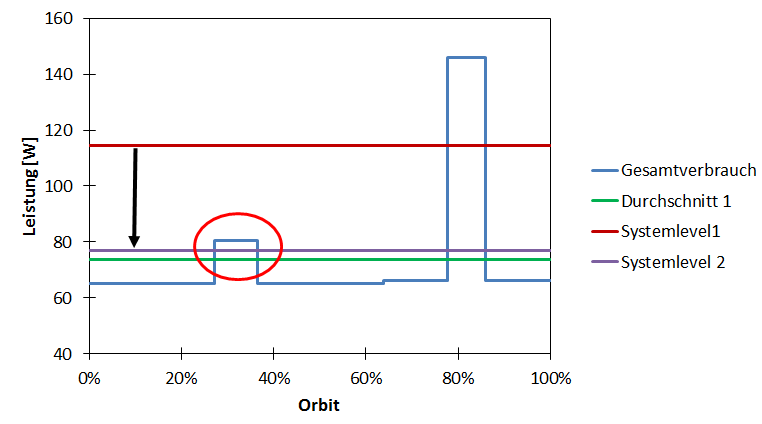
\includegraphics[width=\linewidth]{Fail-Case.png}       
            \caption{Durchschnittlich erfügbare Leistung im System, sowie des Einflusses eines ausgefallenen Paneels und der tatsächliche Verbrauch}
            \label{fig:fail}
         \end{figure}
         Die gesamte für den Wiedereintritt benötigte Leistung (inkl. Boosterzündung) würde die Batterie am EOL auf etwa 50\% entladen. 
%            \begin{table}[H]
%               \centering
%               \begin{tabular}{ccl}
%                  \toprule  
%                  SL. & SSR. & Sub System Requirement \\
%                  \midrule
%                  2 & 1 & \parbox[t]{5cm}{Muss genug Energie für alle Subsysteme im schlechtesten Betriebsfall zur Verfügung stellen können}  \\
%                  %\midrule
%                  3 & 2 & \parbox[t]{5cm}{Batteriekapazität muss für Schattenphasen ausreichend sein}  \\
%                  %\midrule
%                  2 & 3 & \parbox[t]{5cm}{Kapazität für Detumblephase muss ausreichen sein}  \\ 
%                  %\midrule
%                  11 & 4 & \parbox[t]{5cm}{Muss 1 Fehler Tolerant sein}  \\   
%                  %\midrule
%                  6 & 5 & \parbox[t]{5cm}{Muss beim Wiedereintrit genug Energy für De-Orbit, Messungen und Relayfunk bereitstellen köennen}  \\
%                  \bottomrule
%               \end{tabular}
%               \caption{PPS Requirements}
%               \label{tab:ppsreq}
%            \end{table}


         \subsection{S\&M}

         Die Anforderungen an die Struktur sind in erster Linie vom Trägersystem gegben. Dabei werden Abmessungen und Schwerpunktslage so wie Lasten definiert. \\
         Weitere Anforderungen sind eine geringe Masse, gute Zugänglichkeit, Funktionalität und eine geringe Komplexität. Um diese Anforderungen zu erfüllen, wurden verschiedene Konzepte untersucht. Aufgrund der besten Funktionalität wird eine rechteckigen Hybridstruktur aus Aluminium und CFK verwendet. Dieses Konzept bietet gute Festigkeit, ein geringes Gewicht und vorteilhafte thermische Eigenschaften.	\\
         Für die Befestigung der Nutzlast (CHRIS) ist eine optische Bank aus CFK-Sandwich vorgesehen. Hierauf befinden sich auch die Startracker. Durch die geringe thermische Ausdehnung des CFK-Materials sind Verschiebungen zwischen den Startrackern und der Nutzlast minimal, was eine bessere Genauigkeit im Aufnahmemodus ermöglicht. Die optische Bank selbst, wird auf 3 im 60$^\circ$ Winkel verdrehten Haltern angebracht.   
         \\
         Beide Solarpaneele sind mit einem Ausklappmechanismus ausgerüstet. Die Paneele sind über einen Mechanismus mit Nylondraht geischert. Dieswer wird druch redundante Heizer verdampf und die Paneele können ausklappen.
         \\
         An den Halterungen der Paneele wird ein Aramid/Epoxidharz-Verbundwerkstoff eingesetzt. Dieser Zersetzt sich bereits bei ca. 250$^\circ$ Celsius. Diese Sollbruchstellen ermöglichen es, die Paneele beim Wiedereintritt ''abzuwerfen''. Dabei wird keine Wärme in den Satelliten transportiert, da Aramid und Epoxid sehr geringe Wärmeleiteigenschaften aufweisen.\\
         Um sicherzustellen, dass die Struktur den Start unbeschadet übersteht, wurden FEM-Analysen mit NX-Ideas durchgeführt. Es wird eine Modal-Analyse so wie 8 Lastfälle nachgewiesen.\\
         Die Lastfälle entstehen durch eine Überlagerung der vom Trägersystem hervorgerufen Lasten. Diese wurden mit einem Sicherheitsfaktor von 1.5 beaufschlagt.\\
         \begin{table}[H]
            \captionsetup{format=plain}
            \centering
            \begin{tabular}{cccc}
               \toprule  
               Fall & Spann. $[\frac{N}{mm^2}]$ & Dehnung & Versch. [mm]\\
               \midrule
               1 & 32.40 & 0.00013 & 0.318\\
               2 & 29.30 & 0.00011 & 0.286\\
               3 & 24.90 & 0.00011 & 0.254\\
               4 & 37.90 & 0.00017 & 0.462\\
               5 & 27.00 & 0.00007 & 0.295\\
               6 & 28.10 & 0.00009 & 0.364\\
               7 & 36.20 & 0.00009 & 0.413\\
               8 & 36.30 & 0.00015 & 0.499\\
               \bottomrule
            \end{tabular}
            \caption{Lastfälle: Maximalwerte für Spannung, Dehnung und Verschiebung der 8 Lastfälle}
            \label{tab:load_case}
         \end{table}  		
         Als kritsche Fälle stellten sich Fall 4 und Fall 8 herraus. Die Lasten in den beiden kritschen Fällen liegen weit unter den zulässigen Werten und sind somit überdimensioniert.\ref{tab:load_case} In einer späteren Entwicklungs-Phase besteht hier Potential für Gewichtseinsparungen.\\	
         Die Modalanalyse zeigt, dass die Eigenfrequenzen der  Struktur höher als 90Hz sind.\ref{tab:modal} Dies erfüllt die Anforderungen des Trägersystems.      
         \begin{table}[H]
            \centering
            \begin{tabular}{cc}
               \toprule  
               Frequenz [Hz] & Richtung \\
               \midrule
               90.08 & lateral   \\
            %\midrule
               132.13 & lateral  \\
            %\midrule 
               141.34 & lateral\\
            %\midrule
               177.73 & lateral\\
               \bottomrule
            \end{tabular}
            \caption{Modalanalyse: Die ersten 4 Eigenfrequenzen der Struktur}
            \label{tab:modal}
         \end{table}
         \subsection{TCS}
         \begin{table}[H]
            \centering
            \begin{tabular}{ccl}
               \toprule  
               SR & SSR. & Sub System Requirement \\
               \midrule
               2 & 1 & \parbox[t]{5cm}{Muss alle Komponenten im zulässigen Temperaturbereich halten}  \\
            %\midrule
               2 & 2 & \parbox[t]{5cm}{Sollte so wenig Strom wie möglich verbrauchen}  \\
            %\midrule
               \bottomrule
            \end{tabular}
            \caption{TCS Requirements}
            \label{tab:tcsreq}
         \end{table}
         Aus den bestimmten Komponenten der anderen Systeme ergeben sich die exakten thermalen Requirements pro Bauteil. 
         Wenn man die Batterie außen vorlässt, ergibt sich ein operativer Temperaturbereich von $0^{\circ}$ bis $40^{\circ}$. 
         Zum überleben genügen $-10^{\circ}$ bis $50^{\circ}$. Die thermale Anforderung der Batterie würde das Gesamtsystem 
         weiter einschränken,
         deshalb wird diese vom Satelliten isoliert (MLI) und mit einem eigenen Radiator und  1W Heizer versehen.
         \begin{figure}[H]
            \captionsetup{format=plain}
            \centering
            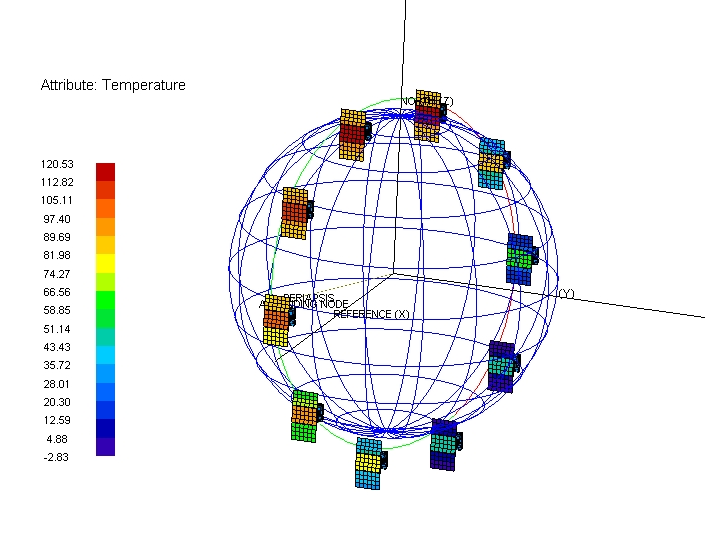
\includegraphics[width=\linewidth]{Orbit_hotcase.png}       
            \caption{Hot Case Orbit Simulation.}
            \label{fig:hotcase}
         \end{figure}
         \begin{figure}[H]
            \captionsetup{format=plain}
            \centering
            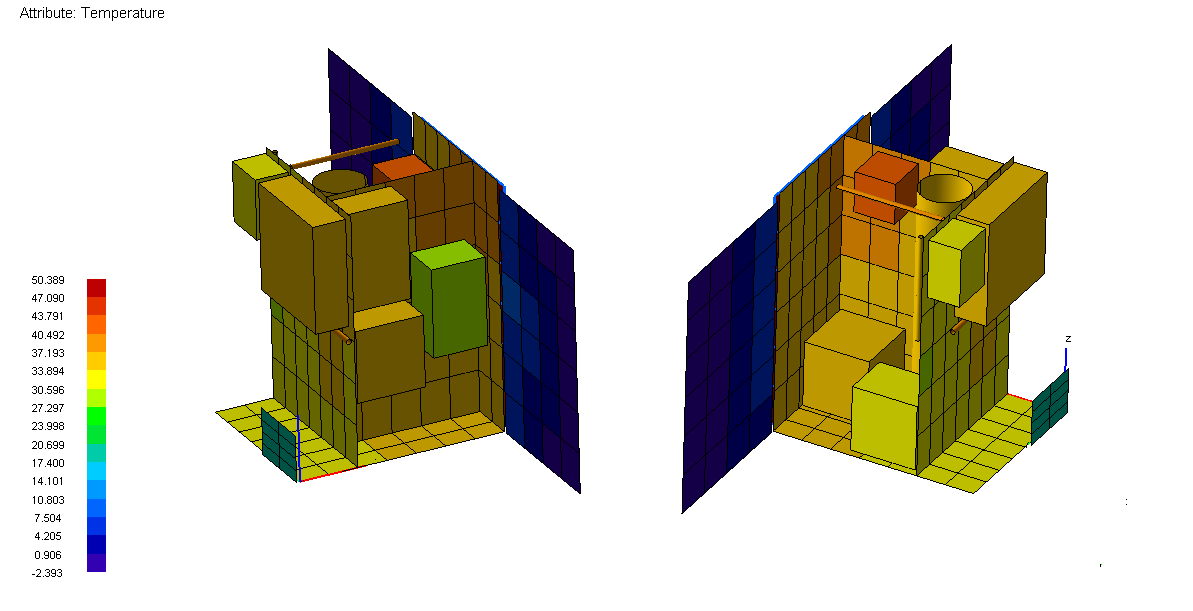
\includegraphics[width=\linewidth]{esatanmodell.png}       
            \caption{Simulations Modell in ESATAN.}
            \label{fig:esatan}
         \end{figure}

         Um vor Sonnen, Albedo und Erd-IR Strahlung zu schützen, ist der Satellit in MLI eingepackt. Insgesamt 
         werden 3 Radiatoren mit einer Gesamtfläche von $0.398m^2$ und ein Batterie Radiator mit $0,055m^2$ verbaut.
         Diese Ergaben sich aus ESATAN Simulationen für den Hot Case, so dass sich die Betriebstemperaturen
         der einzelnen Geräte noch im zulässigen operativen Bereich bewegen. Die selbe Radiatorfläche sorgt
         im Cold-Case für Temperaturen von knapp über $0^{\circ}$ Celsius, womit das Groß der Wärmeregelung passiv 
         Betrieben werden kann. Die Batterie ist mit einem separaten Radiator versehen, der weder zur Erde,
         noch zur Sonne zeigt. Ihre Heatwaste beträgt 8W im Hotcase und 6W im Coldcase.
         Mit 1W Heizleistung im Coldcase sie damit immer im effizienten Bereich.
         \begin{figure}[H]
            \captionsetup{format=plain}
            \centering
            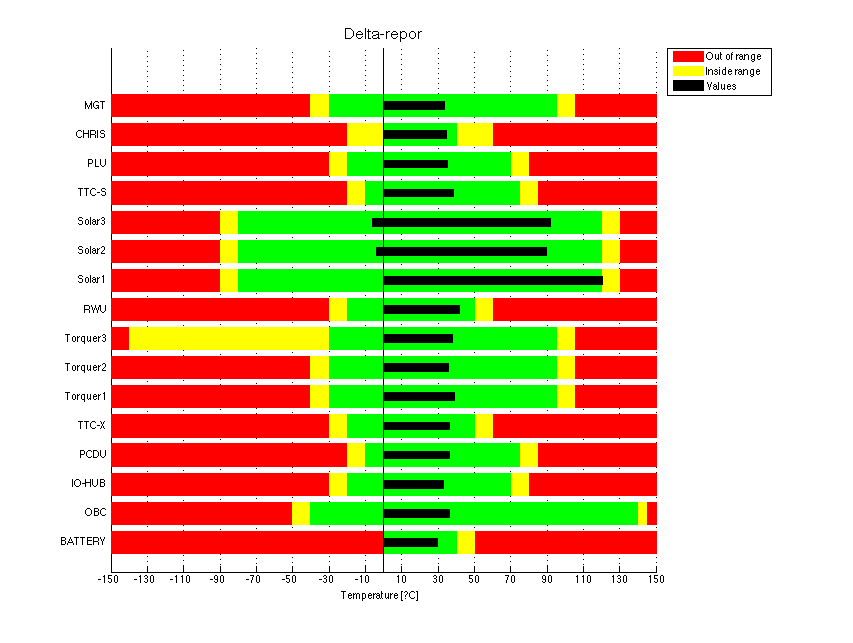
\includegraphics[width=\linewidth]{ThermalBudget.png}       
            \caption{Thermal Budget: Temperaturschwankungen zwischen Hot und Coldcase.}
            \label{fig:thermalbudget}
         \end{figure}

         Zur Überwachung sind im Satelliten 15 Thermoelemente und 15 nahe gelegene Heizer verteilt.
         Diese verhindern im Notfall das Unterkühlen einzelner Komponenten. Im Münchhausen-Fall werden
         sie verwendet, um den Satelliten nach und nach wieder auf Betriebstemperatur zu bringen.
         Figure ref{fig:esatan} zeigt die Orbitansicht der thermalen Simulation für Hot- und Coldcase.
         Das sich Ergebende thermale Budget kann in der Sektion ``System Budgets'' gefunden werden.
         \begin{figure*}[b]
            \captionsetup{format=plain}
            \centering
            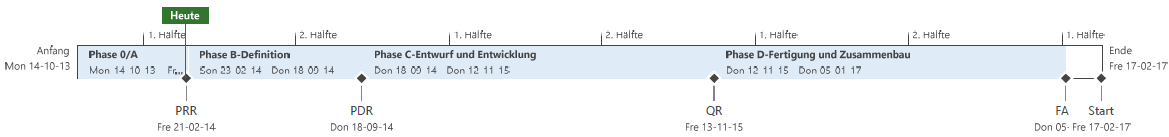
\includegraphics[width=\linewidth]{Zeitachse.png}       
            \caption{Grobe Zeiteinteilung bei der Entwicklung von Nautilus. Die genaue Zeitplanung richtet sich insbesondere nach der Komplexität einzelner zu entwickelnder Komponenten.}
            \label{fig:zeitplan}
         \end{figure*}

%----------------------------------------------------------------------------------------
%	Projekt Planung und Tests
%----------------------------------------------------------------------------------------

         \section{System Budgets}
         Bis auf Temperatur und und Link Budget, wurden alle Größen individuell, nach ihrer Unsicherheit, mit einer Margin von 0\% - 20\% beaufschlagt. Anschließend wurde das Gesamtsystem standardmäßig mit einer Margin von 20\% versehen. Die Ergebnisse für das Gesamtsystem sind in Tab. \ref{tab:bduget_mass_kosten} sichtbar.\\

      %Tabelle Link Budget

         \begin{table}[H]
            \centering
            \begin{tabular}{lrr}
               \toprule    
               & \textbf{Masse [kg}] & \textbf{Preis [\euro]}\\
               \midrule
               \midrule
               \textbf{S\&M} & 30,756 & 100.000,00\\
               \textbf{AOCS}  & 7,810 & 335.400,00\\
               \textbf{OBDH} & 10,700 & 645.044,83\\
               \textbf{PSS} & 15,694 & 512.000,00\\
               \textbf{TT\&C} & 11,106 & 767.613,16\\
               \textbf{TCS} & 2,114 & 75.000,00\\
               \textbf{Prim, Payload} & 14,000 & -\\
               \textbf{Sek, Payload} & 11,292 & -\\
               \textbf{Kabelgewicht} &  11,283 & 50.000,00\\
               \textbf{Zusätzliche Kosten} &  & \\
               \midrule
               Personalkosten &  & 540.000,00\\
               Schütteltest &  & 25.000,00\\
               TV-Test &  & 80.000,00\\
               Komponententest &  & 50.000,00\\
               EMA-Test &  & 25.000,00\\
               SCOE &  & 100.000,00\\
               Kosten X-Band Betrieb &  & 15.000,00\\
               \midrule
               \midrule
               \textbf{Total} & \textbf{114,969} & \textbf{3.320.057,99}\\
               \midrule
               \textbf{+20\% Margin} & \textbf{137,963} & \textbf{3.984.069,59}\\
               \bottomrule 
            \end{tabular}
            \caption{Massen- und Kosten-Budgets}
            \label{tab:bduget_mass_kosten}
         \end{table}

         \section{Projekt Planung und Tests}
         Da der Start im Februar 2017 stattfinden soll, muss sichergestellt sein, dass bis dahin der Satellite voll integriert und alle Bauteile Weltraum qualifiziert wurden. 
         Hierzu wird eine Mischung aus Ingeniers- und Flugmodellen für das finale Konzept verwendet. Die ungefähre Zeitplanung bis zum Start ist in Abb. \ref{fig:zeitplan} dargestellt.

         \begin{thebibliography}{99} % Bibliography - this is intentionally simple in this template

               \bibitem[Wertz, James R. and Larson, Wiley J., 1999]{Larson:1999}
               \newblock Space Mission Analysis and Design, 3rd edition.
               \newblock {\em Space Technology Library}, Volume 8.


         \end{thebibliography}

%----------------------------------------------------------------------------------------

      \end{multicols}

      \end{document}
